\documentclass{scrartcl}
\usepackage[utf8]{inputenc}
\usepackage{verbatim}
\usepackage{enumitem}
\usepackage{graphicx}
\usepackage[ngerman]{babel}
\usepackage{hyperref}
\usepackage[acronym,xindy,toc,nonumberlist]{glossaries} % nomain, if you define glossaries in a file, and you use \newglossaryentry{Client-Server-Architektur} 
	{
	name=Client-Server-Architektur,
	description={Konzept zur Verteilung von Aufgaben in Netzwerken. }
	}
	
	\newglossaryentry{Server} 
	{
	name=Server,
	description={Ein Server kommuniziert mit einem Client, um Aufgaben/Anfragen vom Client zu bearbeiten. }
	}
	
	\newglossaryentry{Client} 
	{
	name=Client,
	description={Ein Client kann Aufgaben/Anfragen an einen Server schicken. }
	}	
	
	\newglossaryentry{Tomcat} 
	{
	name=Tomcat,
	description={Tomcat führt in Java geschriebene Web-Anwendungen auf Servern aus. }
	}	
	
	\newglossaryentry{Android} 
	{
	name=Android,
	description={Android ist ein weitverbreitetes Betriebssystem für Smartphones, welches von Google entwickelt wurde.}
	}	
	
	\newglossaryentry{Gruppengrnder} 
	{
	name=Gruppengründer,
	description={Bezeichnet den Status des Mitglieds, das die Gruppe gegründet hat.}
	}
	
	\newglossaryentry{Mitglied}
	{
	name=Mitglied,
	description={Benutzer der einer Gruppe angehört.}
	}
	
	\newglossaryentry{Teilnehmer}
	{
	name=Teilnehmer,
	description={Ein Mitglied, das an einem Termin teilnimmt}
	}
\makeglossaries
\usepackage[xindy]{imakeidx}
\makeindex
\loadglsentries[main]{INP-00-glossary}
\title{Android Go App - Pflichtenheft}
\author{Jörn Kussmaul, Katharina Riesterer, Julian Neubert,\\ Jonas Walter, Tobias Ohlsson, Eva-Maria Neumann}

\begin{document}
		
	

	\maketitle
	\newpage
	
	\tableofcontents
	\newpage
	%TODO Google Services
	\section{Zielbestimmung}
	Das Ziel ist es eine Android-Applikation zu entwickeln die Gruppen sozialaktiver Menschen eine Plattform bieten soll um kurzfristig Termine zu vereinbaren und bei diesen ein einfaches finden der Gruppe, ohne weitere Kommunikation zu ermöglichen.
	\subsection{Musskriterien}
	\begin{itemize}
		\item Anmeldung mit Google Services
		\item Ein User kann Mitglied mehrerer Gruppen sein und kann Name, Mitglieder, Gründer und Termine einsehen.
		\item Gruppenverwaltung
		\begin{itemize}
			\item Erstellen neuer Gruppen.
			\item Suche bestehender Gruppen.
			\item Gründer-Benutzer-Rollenstruktur.
			\item Mitglieder in die Gruppe aufnehmen, aus der Gruppe entfernen.
			\item Gruppe löschen
			\item Gruppenname ändern
		\end{itemize}
		\item Terminverwaltung
		\begin{itemize}
			\item Termine können mit Zeit, Ort, Name innerhalb einer Gruppe erstellt werden.
			\item User können bei Terminen zu-/absagen.
			\item User werden an ihren Termin erinnert.
		\end{itemize}
		\item Ein User kann seinen eigenen Standort und den Gruppenmittelpunkt abrufen.	
	\end{itemize}
	\subsection{Wunschkriterien}
	\begin{itemize}
		\item \grqq{}Bin Los\grqq{} und \grqq{}Bin da\grqq{} und \grqq{}Bin zu spät\grqq{}
		\begin{itemize}
			\item User können per Button signalisieren ob sie bereits zum Treffpunkt unterwegs sind oder diesen sogar schon erreicht haben.
			\item Nur User die Unterwegs sind werden für den Gruppenmittelpunkt beachtet.
			\item User die den Treffpunkt erreicht haben werden für die Berechnung der Gruppenmitte stärker fokussiert.
			\item Benutzer können der Gruppe mitteilen, dass sie zu spät sind.
		\end{itemize}
		\item Gruppenmittelpunkt teilt sich bei Gruppenteilung.
		\item Die Dauer eines Termins kann individuell festgelegt werden.
		\item Individuelle Erinnerung pro Benutzer und pro Termin.
		\item Erinnerung an Termin auch bei geschlossener App.
		\item Termine können gelöscht, geändert und wiederholt werden.
		\item Statistiken über Teilnahme der User speichern.
		\item QR-Code oder Link zum Finden von Gruppen.
		\item Sprachwahl
	\end{itemize}
	\subsection{Abgrenzungskriterien}
	\begin{itemize}
		\item Kein Chat.
		\item User können nicht die Standorte andere User abfragen.
		\item Gründer kann keine neuen Mitglieder suchen.
	\end{itemize}
	
	\newpage
	
	
	
	\section{Produkteinsatz}
	\begin{itemize}	        
		\item Das Produkt soll das spontane Organisieren von Treffen unterstützen. Dazu soll es dem Benutzer möglich sein in einer Gruppe einen Termin zu erstellen, bzw. bei Terminen zu- oder abzusagen.
		\item Kurz vor dem Termin wird dann der Gruppenmittelpunkt angezeigt, um das Finden der anderen Gruppenmitglieder zu erleichtern.
	\end{itemize}
	\subsection{Anwendungsbereich}
	\begin{itemize}	        
		\item Spontane Terminvereinbarung von Gruppen
	\end{itemize}
	\subsection{Zielgruppe}
	\begin{itemize}	        
		\item Alle Studierende und Mitarbeiter am KIT
	\end{itemize}
	\subsection{Betriebsbedingung}
	\begin{itemize}	        
		\item App kann überall eingesetzt werden
		\item Für vollständigen Funktionsumfang benötigt man GPS und eine stabile Internetverbindung
	\end{itemize}
	
	\newpage
	
	
	\section{Produktumgebung}
	\begin{itemize}	        
		\item Eine Client-Server-Architektur
		\item Der Client ist ein Android-Gerät
		\item Die Android-Go App läuft parallel mit anderen Apps auf einem Android-Gerät
	\end{itemize}
	\subsection{Software}
	\begin{itemize}	        
		\item Client: Android ab 4.4
		\item Server: Tomcat 8, MySQL
	\end{itemize}	
	\subsection{Orgware}
	\begin{itemize}	        
		\item Internetverbindung und Standortabfrage
	\end{itemize}
	\subsection{Produktschnittstelle}
	\begin{itemize}	        
		\item Google Maps
		\item Google Services
	\end{itemize}
	\subsection{Referenzgerät}
	\begin{itemize}
		\item Samsung Galaxy S4
		\item Android 5.0.1
	\end{itemize}
	\newpage
	
	
	\section{Funktionale Anforderungen}
	 In diesem Abschnitt sind die Aussagen über die zu efüllenden Eigenschaften und zu erbringende Leistung unserer App vermerkt. Die mit "[WFAxx]" gekenzeichneten Anforderungen beziehen sich auf die Wunschkriterien der App.
	 
	\subsection{Accountverwaltung}
	\begin{itemize}
		\item[FA10] Anmeldung eines Benutzers in der App über Google Services.
		\item[WFA15] Der Benutzer kann zwischen Sprachen wählen.
		\item[FA20] Ersterfassung und Änderung des Benutzernamens.
		
	\end{itemize}
	
	\subsection{Gruppenverwaltung}
	\begin{itemize}
		\item[FA30] Jeder Benutzer kann eine Gruppe erstellen.
		\item[FA35] Ersterfassung und spätere Änderung des Gruppennamens durch den Gruppengründer.
		\item[FA40] Gruppen können über den Gruppennamen gesucht werden.
		\item[FA45] Benutzer können Beitrittsanfragen an eine Gruppe senden.
		\item[FA50] Der Gruppengründer kann Beitrittsanfragen zu der Gruppe verwalten:
		\begin{itemize}
			\item Anfragen bestätigen, wodurch der Anfragende Mitglied der Gruppe wird und die Anfrage gelöscht wird.
		\end{itemize}
		\begin{itemize}
			\item Anfragen ablehnen, wodurch die Anfrage gelöscht wird.
		\end{itemize}
		\begin{itemize}
			\item Anfragen ignorieren, wodurch die Anfrage bestehen und sichtbar bleibt.
		\end{itemize}
		\item[FA60] Der Gruppengründer kann bestehende Mitglieder aus der Gruppe entfernen.
		\item[FA70] Die Gruppe kann durch den Gruppengründer gelöscht werden.
		\item[FA80] Mitglieder der Gruppen, ausgenommen des Gruppengründers, können die Gruppe verlassen.
		\item[WFA85] Der Gruppengründer kann seinen Status als Gruppengründer an ein Mitglied übergeben.
		\item[FA90] Gruppenmitglieder können andere Gruppenmitglieder anzeigen lassen.
		\item[WFA95] Gruppenmitglieder können die Teilnahmequoten anderer Gruppenmitglieder ansehen.
		
	\end{itemize}
	
	\subsection{Terminverwaltung}
	\begin{itemize}
		\item[FA100] Jedes Mitglied einer Gruppe kann einen Termin erstellen.
		\item[FA110] Der Terminersteller kann den von ihm erstellten Termin verwalten:
		\begin{itemize}
			\item Ersterfassung von Terminnamen, Terminzeit und Terminort.
		\end{itemize}
		
		\begin{itemize}
			\item Visuelle Darstellung des gewählten Terminortes. 
		\end{itemize}
		
		
		\item[WFA115] Der Terminersteller kann den Terminnamen, Terminzeit und Terminort nachträglich ändern oder 				gegebenenfalls löschen.
		
		\item[FA120] Der Termin wird jedem Gruppenmitglied angezeigt.
		\item[FA130] Jedes Gruppenmitglied kann einem Termin zu- oder absagen.
		\item[FA140] Jeder Teilnehmer wird 30 Minuten vor Beginn des Termins benachrichtigt werden.
		\item[WFA145] Teilnehmer werden auch bei geschlossener App benachrichtigt.
		\item[FA150] Der Termin löscht sich eine Stunde nach Ablauf des Terminzeitpunktes automatisch.
		\item[WFA155] Der Zeitpunkt wann der Termin gelöscht wird kann vom Terminersteller beim erstellen des Termins 					bestimmt werden
		
		
	\end{itemize}
	
	\subsection{Terminablauf}
	\begin{itemize}
		\item[FA160] Jeder Teilnehmer kann den Gruppenstandort ab 15 Minuten in einer Karte darstellen lassen.
		\item[FA165W] Vom Gruppenmittelpunkt entfernte Teilgruppen  erhalten einen eigenen Standort. 
		\item[FA170W] Teilnehmer können mittels eines Buttons Signale an die anderen Teilnehmer senden:
		\begin{itemize}
			\item Sie können signalisieren ob sie bereits unterwegs sind.
			\item Sie können signalisieren ob sie zu spät kommen.
			\item Sie können signalisieren ob sie schon am Terminort angekommen sind.
		\end{itemize}
	\end{itemize}
		
	
	\newpage
	
	
	\section{Produktdaten}
	\begin{itemize}
		\item [D10] \textit{Benutzerdaten:}
		Für jeden Benutzer werden die folgenden Daten gespeichert bzw. erfasst:
		\begin{itemize}
			\item Benutzername
			\newline Ein frei gewählter Name, der den anderen Benutzern der App angezeigt wird.
			\item Standort
			\newline Der aktuelle Standort der Person, damit der gemittelte Standort berechnet werden kann.
			\item Google Services Informationen
			\newline Zur eindeutige Identifizierung der Benutzer
		\end{itemize}
		
		\item [D20] \textit{Gruppendaten:}
		Eine Gruppe hat die folgenden Eigenschaften:
		\begin{itemize}
			\item ID
			\newline ID-Nummer zur eindeutigen internen Identifikation
			\item Name
			\newline Angezeigter Name der Gruppe.
			\item Teilnehmer
			\newline In einer Gruppe sind mehrere Benutzer.
			\item Rechte
			\newline Die Teilnehmer haben verschiedene Rechte. Der Gruppengründer hat mehr Rechte als die anderen Teilnehmer.
			\item Termine
			\newline Eine Gruppe kann mehrere Termine haben.
		\end{itemize}
		
		\item [D30] \textit{Termindaten:}
		In der App gibt es mehrere aktive Termine gleichzeitig. Jeder Termin beinhaltet die folgenden Daten:
		\begin{itemize}
			\item Name
			\newline Der Name des Termins.
			\item Ziel
			\newline Das Ziel ist der Standort, wo das Treffen stattfinden soll.
			\item Teilnehmer Status
			\newline Status des Teilnehmers, ob er zu- oder abgesagt oder noch nicht reagiert hat
			\item Gruppe
			\newline Der Termin gehört zu einer bestimmten Gruppe
			\item Serverzeit
			\newline Datum und Uhrzeit des Treffens
		\end{itemize}
	\end{itemize}
	
	\newpage
	
	
	\section{Qualitative Anforderungen}
	\begin{itemize}
		\item[QA10] Die App soll auf jede Anfrage in durchschnittlich unter 5 Sekunden reagieren.
		\item[QA20] Die App fährt in durchschnittlich unter 10 Sekunden hoch.
		\item[QA30] Jede Funktion der App ist mit höchstens 5 Eingaben vom Startbildschirm zu erreichen.
		\item[QA40] Bei 99\% aller Anwendungen werden Fehler abgefangen und führen nicht zum Absturz der App.
		\item[QA50] Unterstützt bis zu 50 Benutzer pro Gruppe.
		\item[QA60] Jeder Benutzer kann in bis zu 20 Gruppen Mitglied sein.
		\item[QA70] Die App unterstützt mindestens 30000 Benutzer.
	\end{itemize}
	
	\newpage
	
	
	\section{Globale Testfälle}

	Es muss überprüft werden ob folgende Funktionen wie gewünscht funktionieren.
	
	\subsection{Accountverwaltung}
	\begin{itemize} 
		\item[T10] Registrieren: Eine bisher nicht registrierte Person mit einem Google-Account registriert sich mit diesem im System und wählt zusätzlich einen Benutzernamen.
		\item[T20] Namensänderung: Ein Benutzer ändert seinen Benutzernamen.
	\end{itemize}	
	
	\subsection{Gruppenverwaltung}
	\begin{itemize}
		\item[T30] Ein Benutzer erstellt eine neue Gruppe hierzu muss:
			\begin{itemize}
			\item ein Gruppenname eingegeben werden
			\item der entsprechende Benutzer als Gruppengründer eingetragen werden
			\end{itemize}
		\item[T40] Gruppenverwaltung aus Gründersicht:
			\begin{itemize}
			\item der Gründer wirft Mitglieder aus der Gruppe
			\item ändert den Gruppennamen
			\item nimmt Beitrittsanfragen an
			\item löscht Beitrittsanfragen
			\item löscht die Gruppe
			\end{itemize}
		\item[T50] Einer existierende Gruppe beitreten:
	 		\begin{itemize}
			\item ein Benutzer sucht über den Gruppennamen nach einer Gruppe 
			\item schickt der Gruppe eine Beitrittsanfrage
			\item wartet auf eine Reaktion des Gruppengründers
			\item bei einer Annahme ist der Benutzer dann Mitglied der Gruppe
			\item bei einer Ablehnung wird die Beitrittsanfrage gelöscht 
			\end{itemize}
		\item[T60] Gruppe Verlassen: Ein Gruppenmitglied, nicht der Gründer, verlässt eine Gruppe.
	\end{itemize}	

	\subsection{Terminverwaltung}
	\begin{itemize}
		\item[T70] Ein beliebiges Gruppenmitglied erstellt einen neuen Termin hierzu muss:
			\begin{itemize}
			\item ein Terminname eingegeben werden
			\item ein Treffpunkt festgelegt werden
			\item das Datum und die Uhrzeit des Termins festgelegt werden
			\item der entsprechende Benutzer als Terminadministrator und damit auch als Teilnehmer eingetragen werden
			\item der Termin nachdem er vorüber ist gelöscht werden
			\end{itemize}
		\item[WT80] Terminverwaltung durch den Terminadministrator:
			\begin{itemize}
			\item der Terminadministrator ändert den Treffpunkt
			\item den Terminnamen
			\item die Uhrzeit des Termins
			\end{itemize}
		\item[T90] Ein Mitglied lässt sich einen Termin anzeigen und erhält folgende Informationen:
			\begin{itemize}
			\item Terminname, Treffpunkt und Zeitpunkt
			\item wer den Termin gegründet hat
			\item die Liste aller Teilnehmer
			\item nur bei eigener Teilnahme und bei Terminstart: den Gruppenmittelpunkt
			\end{itemize}
		\item[T100] Ein Mitglied sagt bei einem Termin zu daraufhin wird:
			\begin{itemize}
			\item das Mitglied zum Teilnehmer
			\item in die Teilnehmerliste aufgenommen
			\item vor Beginn des Termins benachrichtigt
			\end{itemize}
		\item[T110] Ein Mitglied sagt bei einem Termin ab woraufhin der Termin nicht mehr angezeigt wird. 
	\end{itemize}

	\subsection{Standort}
	\begin{itemize}
		\item[T120] Der Server lokalisiert alle Teilnehmer eines Termins eine viertel Stunde vor Terminbeginn und berechnet den gemittelten Standort. 
		\item[T130] Der Server löscht nach Ende des Termins alle Informationen über die Standorte der Teilnehmer. 
	 \end{itemize}	
	
	\newpage
	
	
	\section{Systemmodelle}
	
	\subsection{Anwendungsfälle}
	\subsubsection{Benutzer Registrieren}
	\begin{description}
		\item \textbf{Titel:}
		\begin{description}
			\item Benutzer Registrieren
		\end{description}
		\item \textbf{Kurzbeschreibung:}
		\begin{description}
			\item Der Benutzer registriert sich mit seinem Google Account.
		\end{description}
		\item \textbf{Aktoren:}
		\begin{description}
			\item Benutzer 
		\end{description}
		\item \textbf{Vorbedingungen:}
		\begin{description}
			\item Der Benutzer besitzt einen Google Account
			\item Mit diesem Google Account ist noch kein Konto verknüpft
		\end{description}
		\item \textbf{Ablauf:} \newline Für den Benutzer wird ein Konto auf der Datenbank erstellt und mit seinem Google Account verknüpft.
		\item \textbf{Ergebnis:} \newline Der Benutzer besitzt ein Konto und kann somit zu Gruppen hinzugefügt werden oder selber Gruppen erstellen.
	\end{description}
	
	\newpage
	
	\subsubsection{Gruppe erstellen}
	\begin{description}
		\item \textbf{Titel:}
		\begin{description}
			\item Gruppe erstellen
		\end{description}
		\item \textbf{Kurzbeschreibung:}
		\begin{description}
			\item Der Benutzer erstellt eine Gruppe.
		\end{description}
		\item \textbf{Aktoren:}
		\begin{description}
			\item Benutzer 
		\end{description}
		\item \textbf{Vorbedingungen:}
		\begin{description}
			\item Der Benutzer hat sich zuvor erfolgreich registriert.
		\end{description}
		\item \textbf{Ablauf:} \newline Es wird eine Gruppe erstellt, für die der erstellende Benutzer als Gründer eingetragen wird. Der Benutzer muss einen Namen für seine Gruppe wählen. Damit erhält der Benutzer auch alle Rechte, die dem Gruppengründer zugestanden werden. 
		\item \textbf{Ergebnis:} \newline Der Benutzer ist Gruppengründer einer Gruppe und kann Benutzer zu dieser Gruppe hinzufügen oder Mitglieder aus der Gruppe entfernen. Des Weiteren hat er die selben Rechte wie Mitglieder, er kann also auch Termine erstellen und an anderen Terminen innerhalb der Gruppe teilnehmen.
	\end{description}
	
	\newpage
	
	\subsubsection{Benutzer hinzufügen}
	\begin{description}
		\item \textbf{Titel:}
		\begin{description}
			\item Benutzer hinzufügen
		\end{description}
		\item \textbf{Kurzbeschreibung:}
		\begin{description}
			\item Der Gruppengründer fügt Benutzer hinzu.
		\end{description}
		\item \textbf{Aktoren:}
		\begin{description}
			\item Gruppengründer
			\item Benutzer
		\end{description}
		\item \textbf{Vorbedingungen:}
		\begin{description}
			\item Der Gruppengründer hat zuvor eine Gruppe gegründet und der Benutzer hat sich bereits registriert.
		\end{description}
		\item \textbf{Ablauf:} \newline Der Benutzer kann nach der Gruppe des Gruppengründers suchen und eine Beitrittsanfrage senden. Wurde die Anfrage gesendet kann der Gruppengründer sie einsehen und den Benutzer annehmen oder ablehnen. Hat der Gruppengründer den Benutzer angenommen ist der Benutzer nun Mitglied in der Gruppe und hat alle Rechte eines Mitglieds.
		\item \textbf{Ergebnis:} \newline Der Benutzer ist Mitglied einer Gruppe und kann Termine erstellen oder an von anderen Personen innerhalb der Gruppe erstellten Terminen teilnehmen.
	\end{description}
	
	\newpage
	
	\subsubsection{Termin erstellen}
	\begin{description}
		\item \textbf{Titel:}
		\begin{description}
			\item Termin erstellen
		\end{description}
		\item \textbf{Kurzbeschreibung:}
		\begin{description}
			\item Ein Mitglied erstellt einen Termin.
		\end{description}
		\item \textbf{Aktoren:}
		\begin{description}
			\item Mitglied
		\end{description}
		\item \textbf{Vorbedingungen:}
		\begin{description}
			\item Das Mitglied ist Mitglied einer Gruppe
		\end{description}
		\item \textbf{Ablauf:} \newline Das Mitglied erstellt innerhalb einer Gruppe einen Termin. Hierfür gibt er Namen, Uhrzeit und Ort für den Termin an. Das Mitglied, das den Termin erstellt nimmt automatisch an dem Termin teil. Der Termin ist und die Gruppe gebunden und alle anderen Mitglieder der Gruppe können die Informationen für diesen Termin einsehen und ihm beitreten.
		\item \textbf{Ergebnis:} \newline Das Mitglied hat einen an die Gruppe gebunden, für alle Mitglieder sichtbaren Termin erstellt. Mitglieder können an dem Termin als Teilnehmer beitreten. Ein Teilnehmer wird eine gewisse Zeit vor dem Termin benachrichtigt. Wurde der Teilnehmer benachrichtigt kann er die Karte öffnen und den ungefähren Standort der anderen Teilnehmer dieses Termins einsehen.
	\end{description}
	
	\newpage
	
	\subsection{Anwendungsfalldiagramm}
	\begin{figure}[h]
		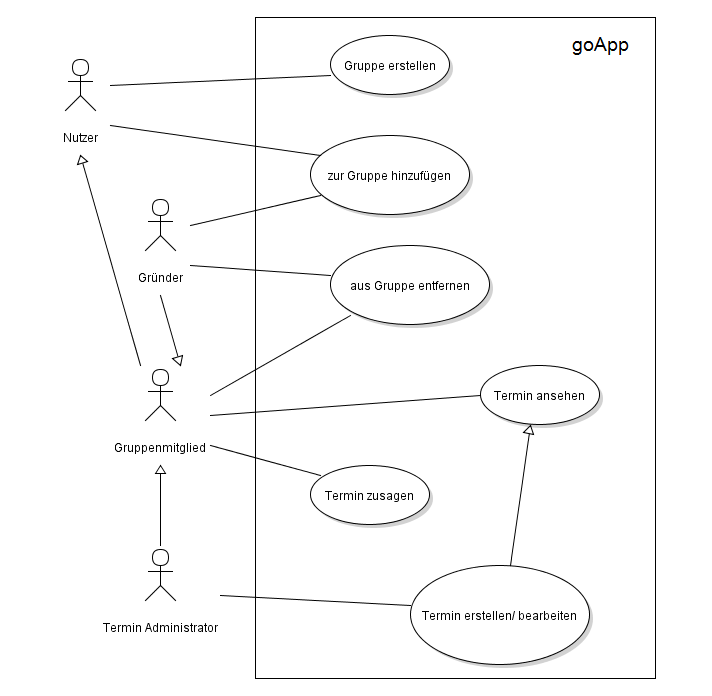
\includegraphics[width=\textwidth]{goApp_useCase}
	\end{figure}
	
	\newpage
	
	\subsection{Szenarien}
	\subsubsection{Szenario 1}
	Alice, Bob und Carol gehen oft gemeinsam in der Mensa essen. Zur besseren Koordination haben sie die App auf ihren Android-Smartphones installiert.
	Nun startet jeder bei sich die App und gibt, nachdem er sich über sein Google Konto angemeldet hat, seinen Namen ein.
	Alice gründet nun eine neue Gruppe mit dem Namen ABC-Mensa. Danach geben Bob und Carol in das Suchfeld ABC-Mensa ein und klicken auf die entsprechende Gruppe.
	Es erscheint nun auf dem Display die Nachfrage ob sie der Gruppe beitreten wollen. Sobald sie dies bestätigt haben klickt Alice auf die Gruppe,
	sieht die Namen Bob und Carol als Bewerber, und fügt beide hinzu.
	Bob bekommt nun Hunger, klickt auf die Gruppe und erstellt einen neuen Termin mit dem Namen Mensa, dem entsprechenden Datum, der Uhrzeit 12:30 und dem Ort der Mensa.
	Kurze Zeit darauf schauen Alice und Carol auf ihr Smartphone, sehen den Termin und klicken beide auf \glqq{}Teilnehmen\grqq{}.
	Um 12:15 erscheint auf allen Smartphones die Benachrichtigung, dass in 15 Minuten der Termin ansteht.
	Alle gehen kurz daraufhin los und können in der App sowohl ihren als auch den mittleren Gruppenstandort sehen.
	Nachdem der Termin vorbei ist, wird er automatisch gelöscht.
	\newline
	\newline
	\begin{figure}[h]
	\centering
	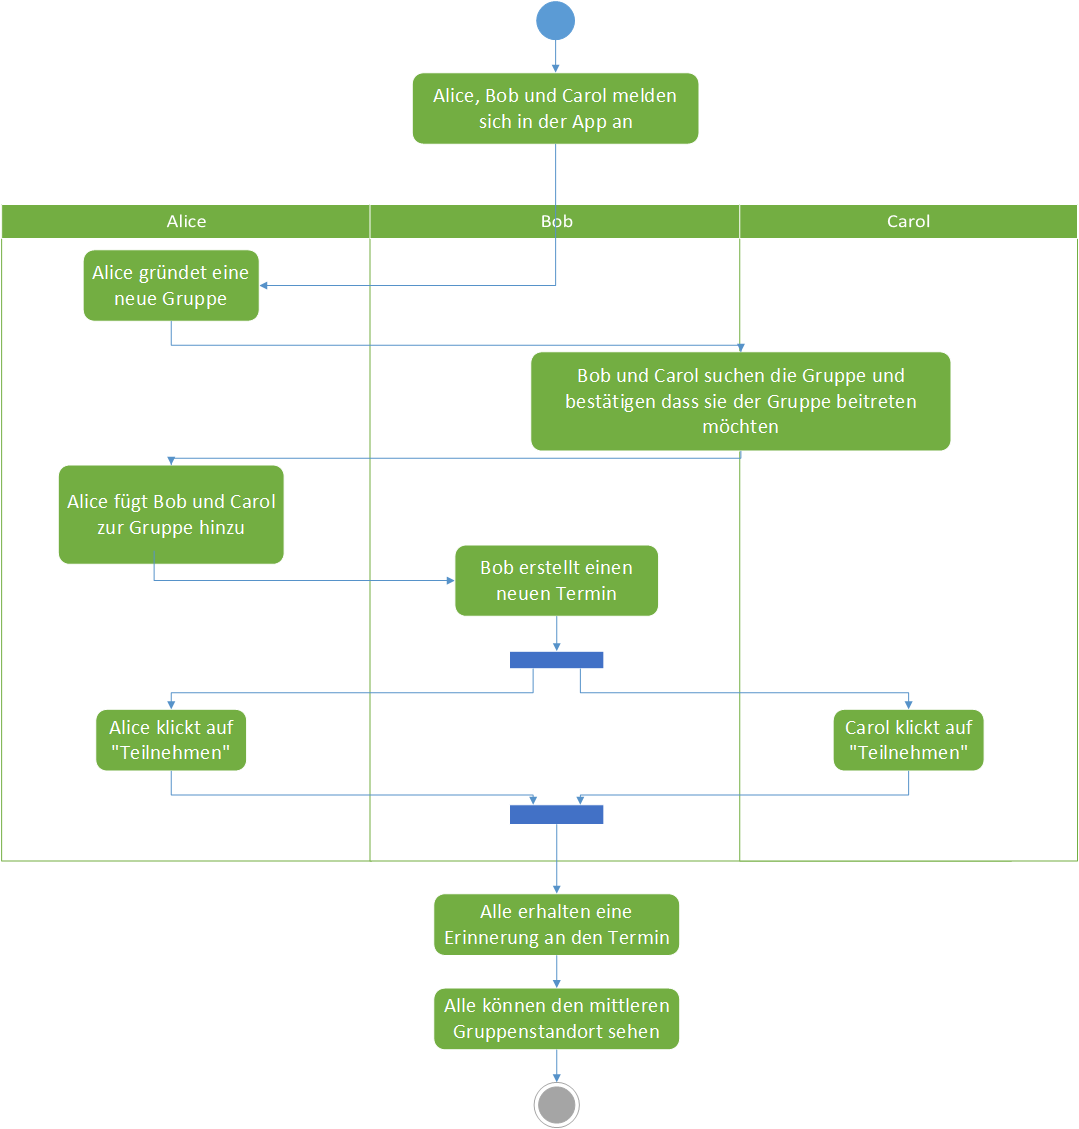
\includegraphics[width=\textwidth]{Szenario1}
	\end{figure}
	
	\newpage
	
	
	\subsubsection{Szenario 2}
	Die Personen Alice, Bob, Carol, Dave und Eve sind in einer gemeinsamen Gruppe.
	Alice will um 12:00 Uhr in die Mensa gehen. Daher erstellt Alice in der Gruppe einen neuen Termin \glqq{}Mensa 12:00\grqq{}.
	Alle anderen Gruppenmitglieder sehen den neuen Termin. Bob und Carol wollen auch um 12:00 in die Mensa gehen und klicken auf \glqq{}Teilnehmen\grqq{}.
	Dave und Eve müssen um 12:00 Uhr noch etwas erledigen und können deshalb erst später in die Mensa, sie klicken deshalb auf \glqq{}Nicht Teilnehmen\grqq{}.
	Da sie auf \glqq{}Nicht Teilnehmen\grqq{} geklickt haben, ist der Termin für sie nicht mehr sichtbar.
	Dave erstellt später einen neuen Termin \glqq{}Mensa 12:30\grqq{} in der Gruppe.
	Um 12:30 hat Eve auch Zeit und klickt auf \glqq{}Teilnehmen\grqq{}.
	Da Alice, Bob und Carol schon früher in die Mensa gehen klicken sie auf \glqq{}Nicht Teilnehmen\grqq{}.
	Um 11:45 werden Alice, Bob und Carol an ihren Termin erinnert und um 12:15 Dave und Eve.
	Der mittlere Gruppenstandort bezieht sich immer ausschließlich auf die Personen, die an dem Termin teilnehmen.
	So sieht Alice den mittleren Standort von sich, Bob und Carol.	
	\newline
	\newline
	\newline
	\begin{figure}[h]
		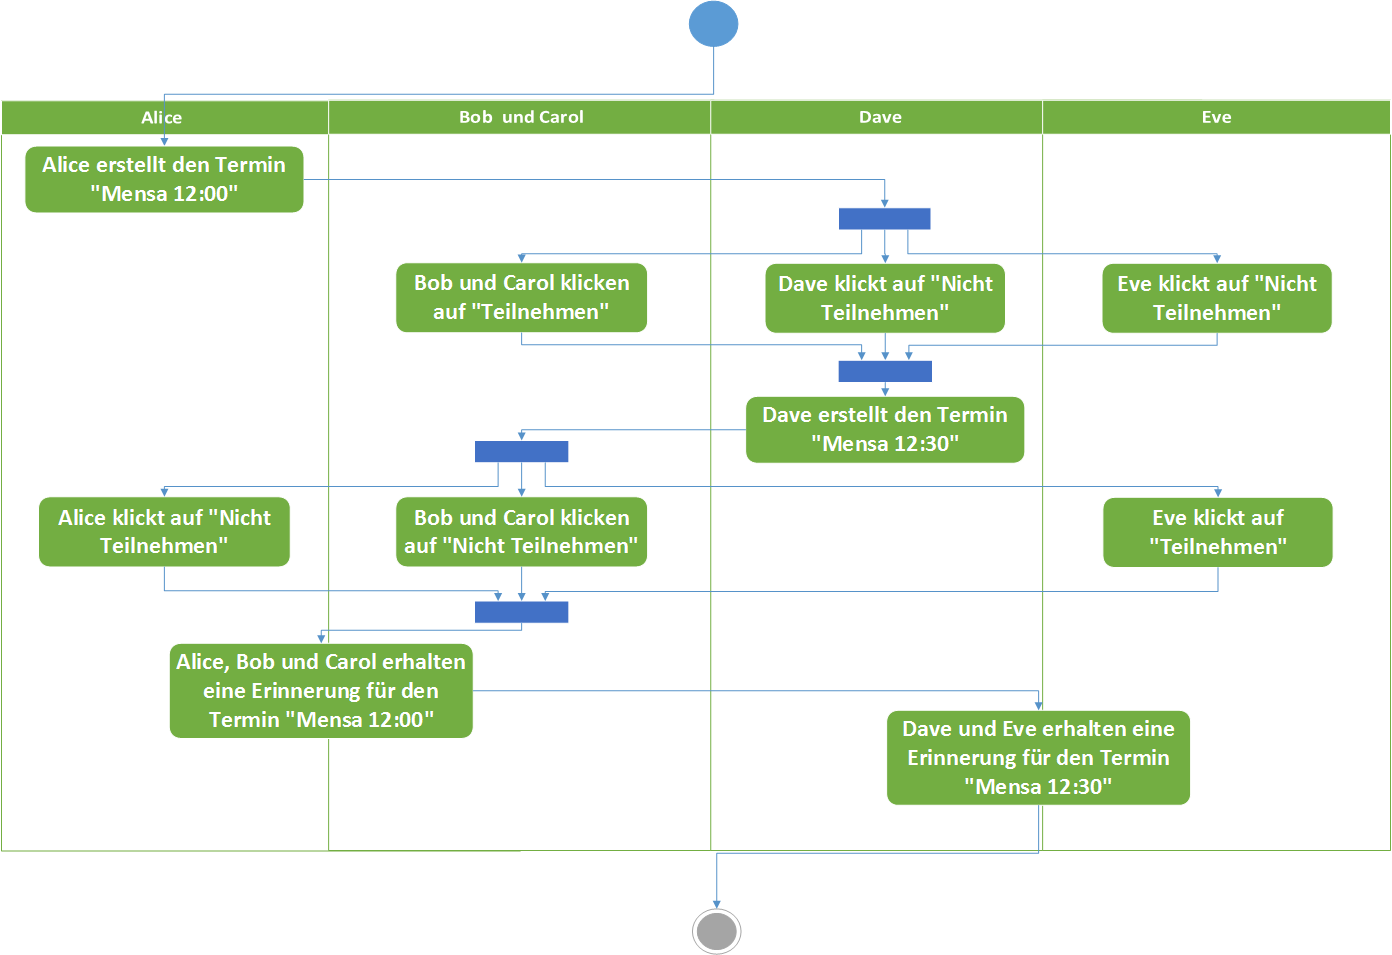
\includegraphics[width=\textwidth]{Szenario2}
	\end{figure}
	\newpage
	
	\subsubsection{Szenario 3}
	Es gibt die Personen Alice, Bob, Carol und Dave, welche alle bereits in der App registriert sind.
	Alice hat Geburtstag und erstellt deshalb eine neue Gruppe mit dem Namen \glqq{}Geburtstag Alice\grqq{}. Die anderen geben in das Suchfeld \glqq{}Geburtstag Alice\grqq{} ein und klicken auf die passende Gruppe.
	Jetzt erscheint die Nachfrage, ob sie der Gruppe beitreten wollen. Alice sieht nun, welche von ihren Gästen teilnehmen wollen und fügt diese hinzu. Dave möchte auch beitreten, aber Alice hat ihn nicht eingeladen und lehnt seine Anfrage ab.
	Sobald alle Gäste der Gruppe beigetreten sind, erstellt Alice einen neuen Termin mit dem Namen \glqq{}Feier\grqq{} und ihrem zu Hause als Ort, sowie dem Datum \glqq{}27.11.2016\grqq{} und die Uhrzeit \glqq{}21:00\grqq{}.
	Bob und Carol sehen den Termin und klicken auf \glqq{}Teilnehmen\grqq{}.
	%TODO Erinnerung: Um 12:15 erscheint auf allen Smartphones die Benachrichtigung, dass in 15 Minuten der Termin ansteht. Alle gehen kurz daraufhin los und können in der App sowohl ihren als auch den mittleren Gruppenstandort sehen.
	Nachdem der Termin vorbei ist, wird er automatisch gelöscht.
	Am nächsten Tag verlässt Bob die Gruppe und Alice löscht daraufhin die Gruppe, da sie nicht mehr gebraucht wird.	
	\newline
	\newline
	\begin{figure}[h]
		\centering
		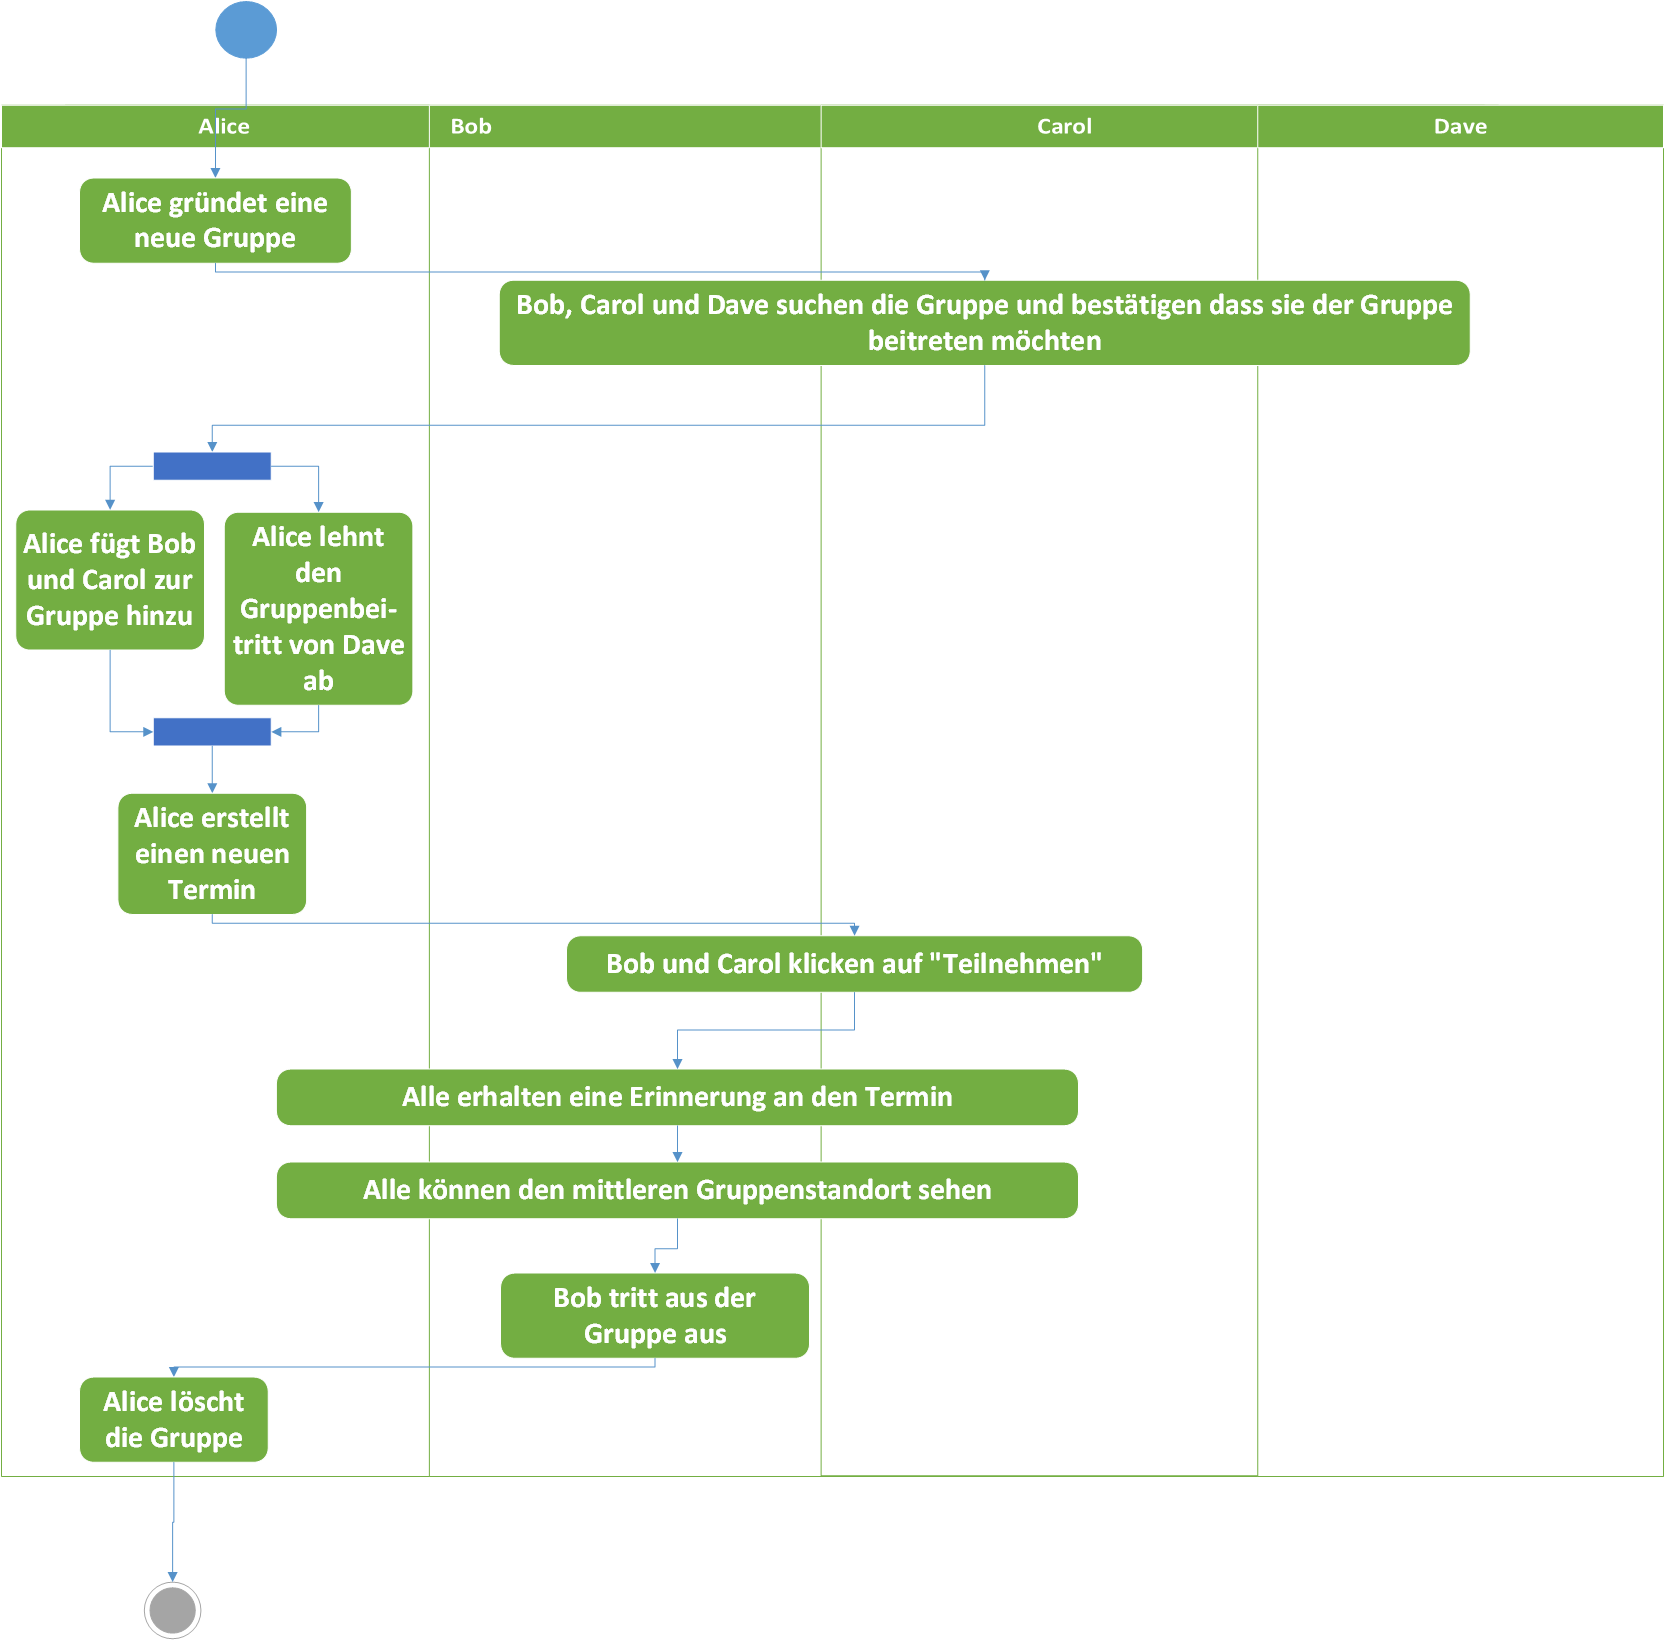
\includegraphics[width=0.9\textwidth]{Szenario3}
	\end{figure}
	\newpage
	
	\subsubsection{Szenario 4 (Wunschszenario)}
	Alice, Bob, Carol und Dave wollen sich am Abend im Restaurant \glqq{}Oxford\grqq{} in Karlsruhe zum Essen treffen. 
	Da sie alle die Android Go App installiert haben und einer gemeinsamen Gruppe angehören, erstellt Alice in der App 		einen Termin names \glqq{}Oxford\grqq{}, dem die drei anderen zusagen. Alice trifft Bob pünktlich um 8:00 Uhr im 		\glqq{}Oxford Pub\grqq{} kann jedoch Carol und Dave nicht finden, die in der App durch den \glqq{}Bin da\grqq{}-Button 		jedoch schon signalisiert haben vor Ort zu sein. Deshalb öffnet Alice die Go App und versucht über den Gruppenstandort 		mehr Information zu erhalten. Carol und Dave haben sich inzwischen in dem 200 Meter entfernten \glqq{}Oxford 			\grqq{} getroffen. Alice erkennt in der Karte der App durch die Clusteringanalyse neben dem Standort von ihr und 		Bob einen zweiten Standort, der zu Carol und Dave gehören muss. Sie bemerkt dadurch das Missverständnis zwischen 		\glqq{}Oxford Pub\grqq{} und \glqq{}Oxford Cafe\grqq{} sofort und macht sich mit Bob in Richtung \glqq{}Oxford 			Cafe\grqq{} auf.    
	
	
	
	
	
	
	
	
	\newpage
	
	\subsection{GUI}
	\begin{figure}[h]
		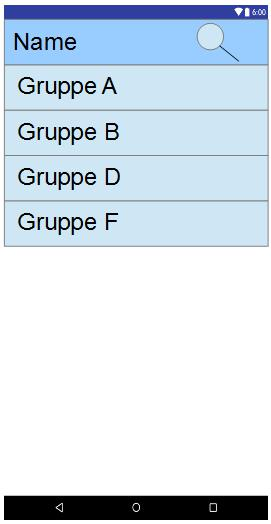
\includegraphics[width=.5\textwidth]{GUI_Start.jpg}
		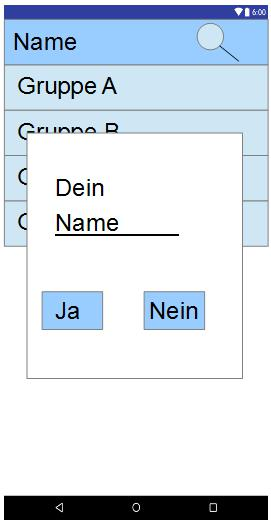
\includegraphics[width=.5\textwidth]{GUI_changeName.jpg}
		\caption{Die Startseite zeigt den Namen des Benutzers und bietet eine Übersicht über alle Gruppen in denen der Benutzer Mitglied ist. Außerdem lässt sich hier der eigene Anzeigename ändern.}
	\end{figure}
	
	\newpage
	\begin{figure}[h]
		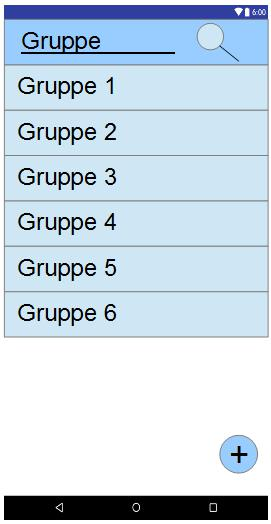
\includegraphics[width=.5\textwidth]{GUI_NeueGruppe.jpg}
		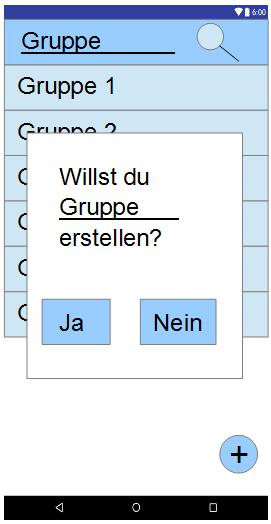
\includegraphics[width=.5\textwidth]{GUI_GruppeNeuBest.jpg}
		\caption{Die Gruppensuche zeigt dem Benutzer alle Gruppen an deren Name mit seiner Eingabe startet, zusätzlich kann der Benutzer hier eine neue Gruppe erstellen.}
	\end{figure}
	
	\newpage
	\begin{figure}[h]
		\centering
		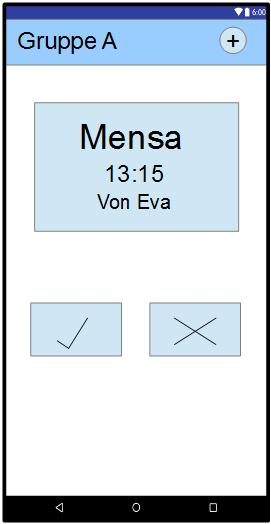
\includegraphics[width=.5\textwidth]{GUI_Gruppe.jpg}
		\caption{In einer Gruppe bekommt ein  Mitglied die Termine der Gruppe angezeigt und kann bei diesen zu- oder absagen, mit einem wischen kann zwischen allen aktuellen Terminen gewechselt werden. Es kann ebenfalls ein eigener Termin erstellt und weitere Details sowohl über die Gruppe als auch die Termine abgerufen werden.}
	\end{figure}
	
	\newpage
	\begin{figure}[h]
		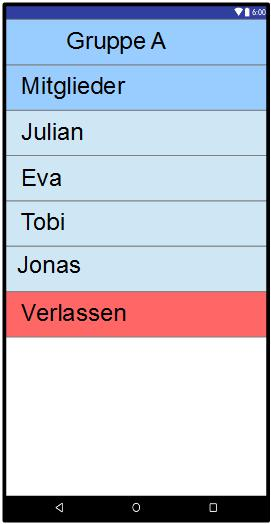
\includegraphics[width=.5\textwidth]{GUI_GruppeInfoNormal.jpg}
		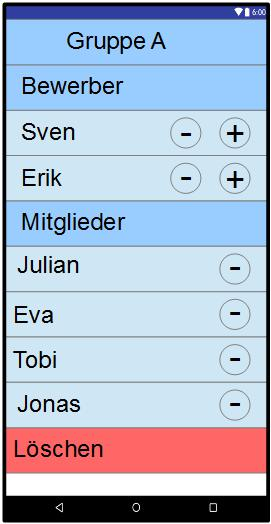
\includegraphics[width=.5\textwidth]{GUI_GruppeInfoGruender.jpg}
		\caption{In der Gruppeninformationsansicht sehen Mitglieder alle anderen Mitglieder der Gruppe und sie können die Gruppe verlassen. Der Gründer der Gruppe kann zusätzlich einzelne Mitglieder aus der Gruppe entfernen und Beitrittsanfragen bearbeiten, anstatt die Gruppe zu verlassen kann er die Gruppe löschen.}
	\end{figure}
	
	\newpage
	\begin{figure}[h]
		\centering
		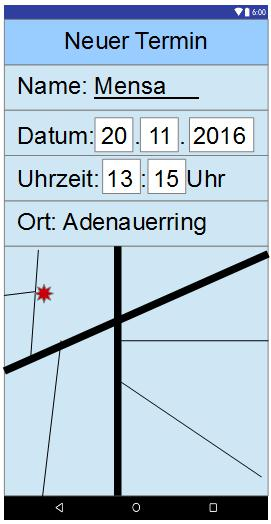
\includegraphics[width=.5\textwidth]{GUI_NeuerTermin.jpg}
		\caption{Damit ein Mitglied einen neuen Termin erstellen kann muss es dem Termin einen Namen geben und ihn mit Datum, Uhrzeit und einem Ort versehen.}
	\end{figure}
	
	\newpage
	\begin{figure}[h]
		\centering
		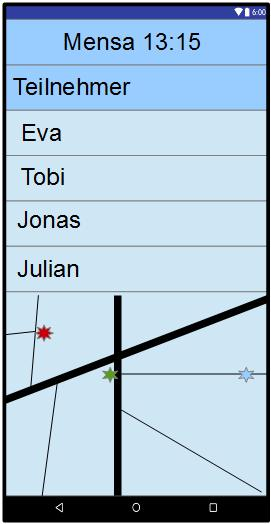
\includegraphics[width=.5\textwidth]{GUI_Termin.jpg}
		\caption{In der Terminansicht erhält ein Mitglied alle Informationen über einen Termin, darunter sind eine Teilnehmerliste und eine Karte die den Treffpunkt und den eigenen Standort anzeigt. Sollte der Termin kurz bevorstehen wird zusätzlich der gemittelte Gruppenstandort angezeigt.}
	\end{figure}
	


\appendix
\bibliographystyle{plainnat}
\bibliography{bibtex}
\printindex
\glsaddall
\printglossaries
	
\end{document}
